%!TEX root = ../main.tex
\vspace{-0.5em}
\subsection{Convergence Evaluation}

\begin{figure}[t]   
	\centering
	\begin{minipage}[t]{0.49\textwidth}
		\centering
		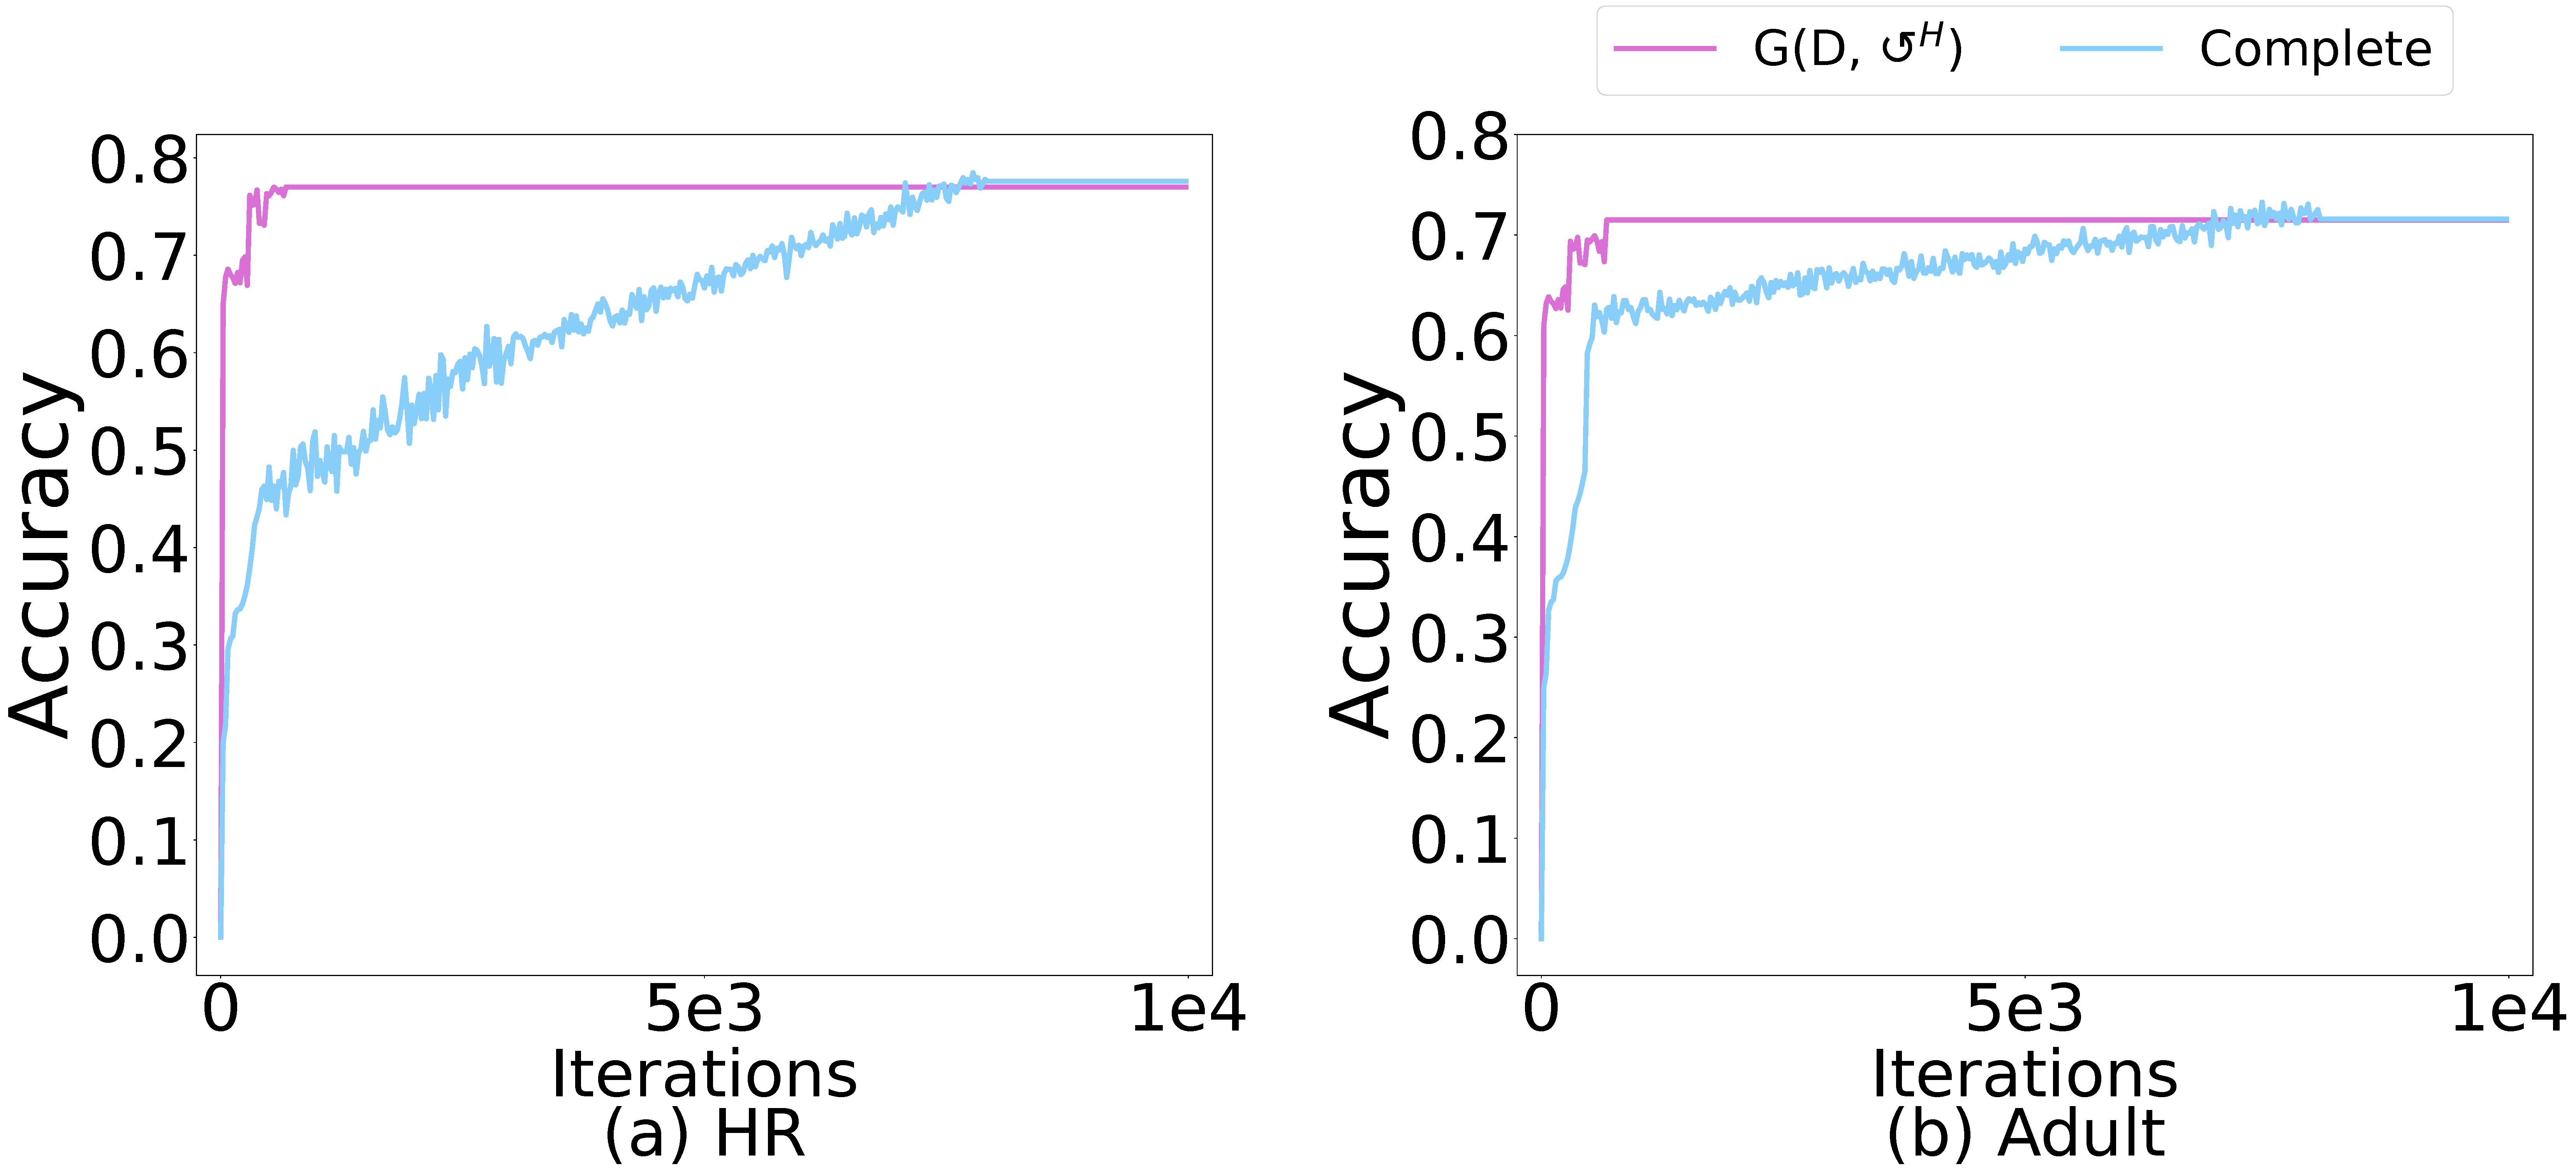
\includegraphics[width=\columnwidth]{figs/G_a}
	    \vspace{-1.5em}
		\caption{Convergence of \ours.}
		\label{fig:converge_G}
	\end{minipage}
	\begin{minipage}[t]{0.49\textwidth}
		\centering
		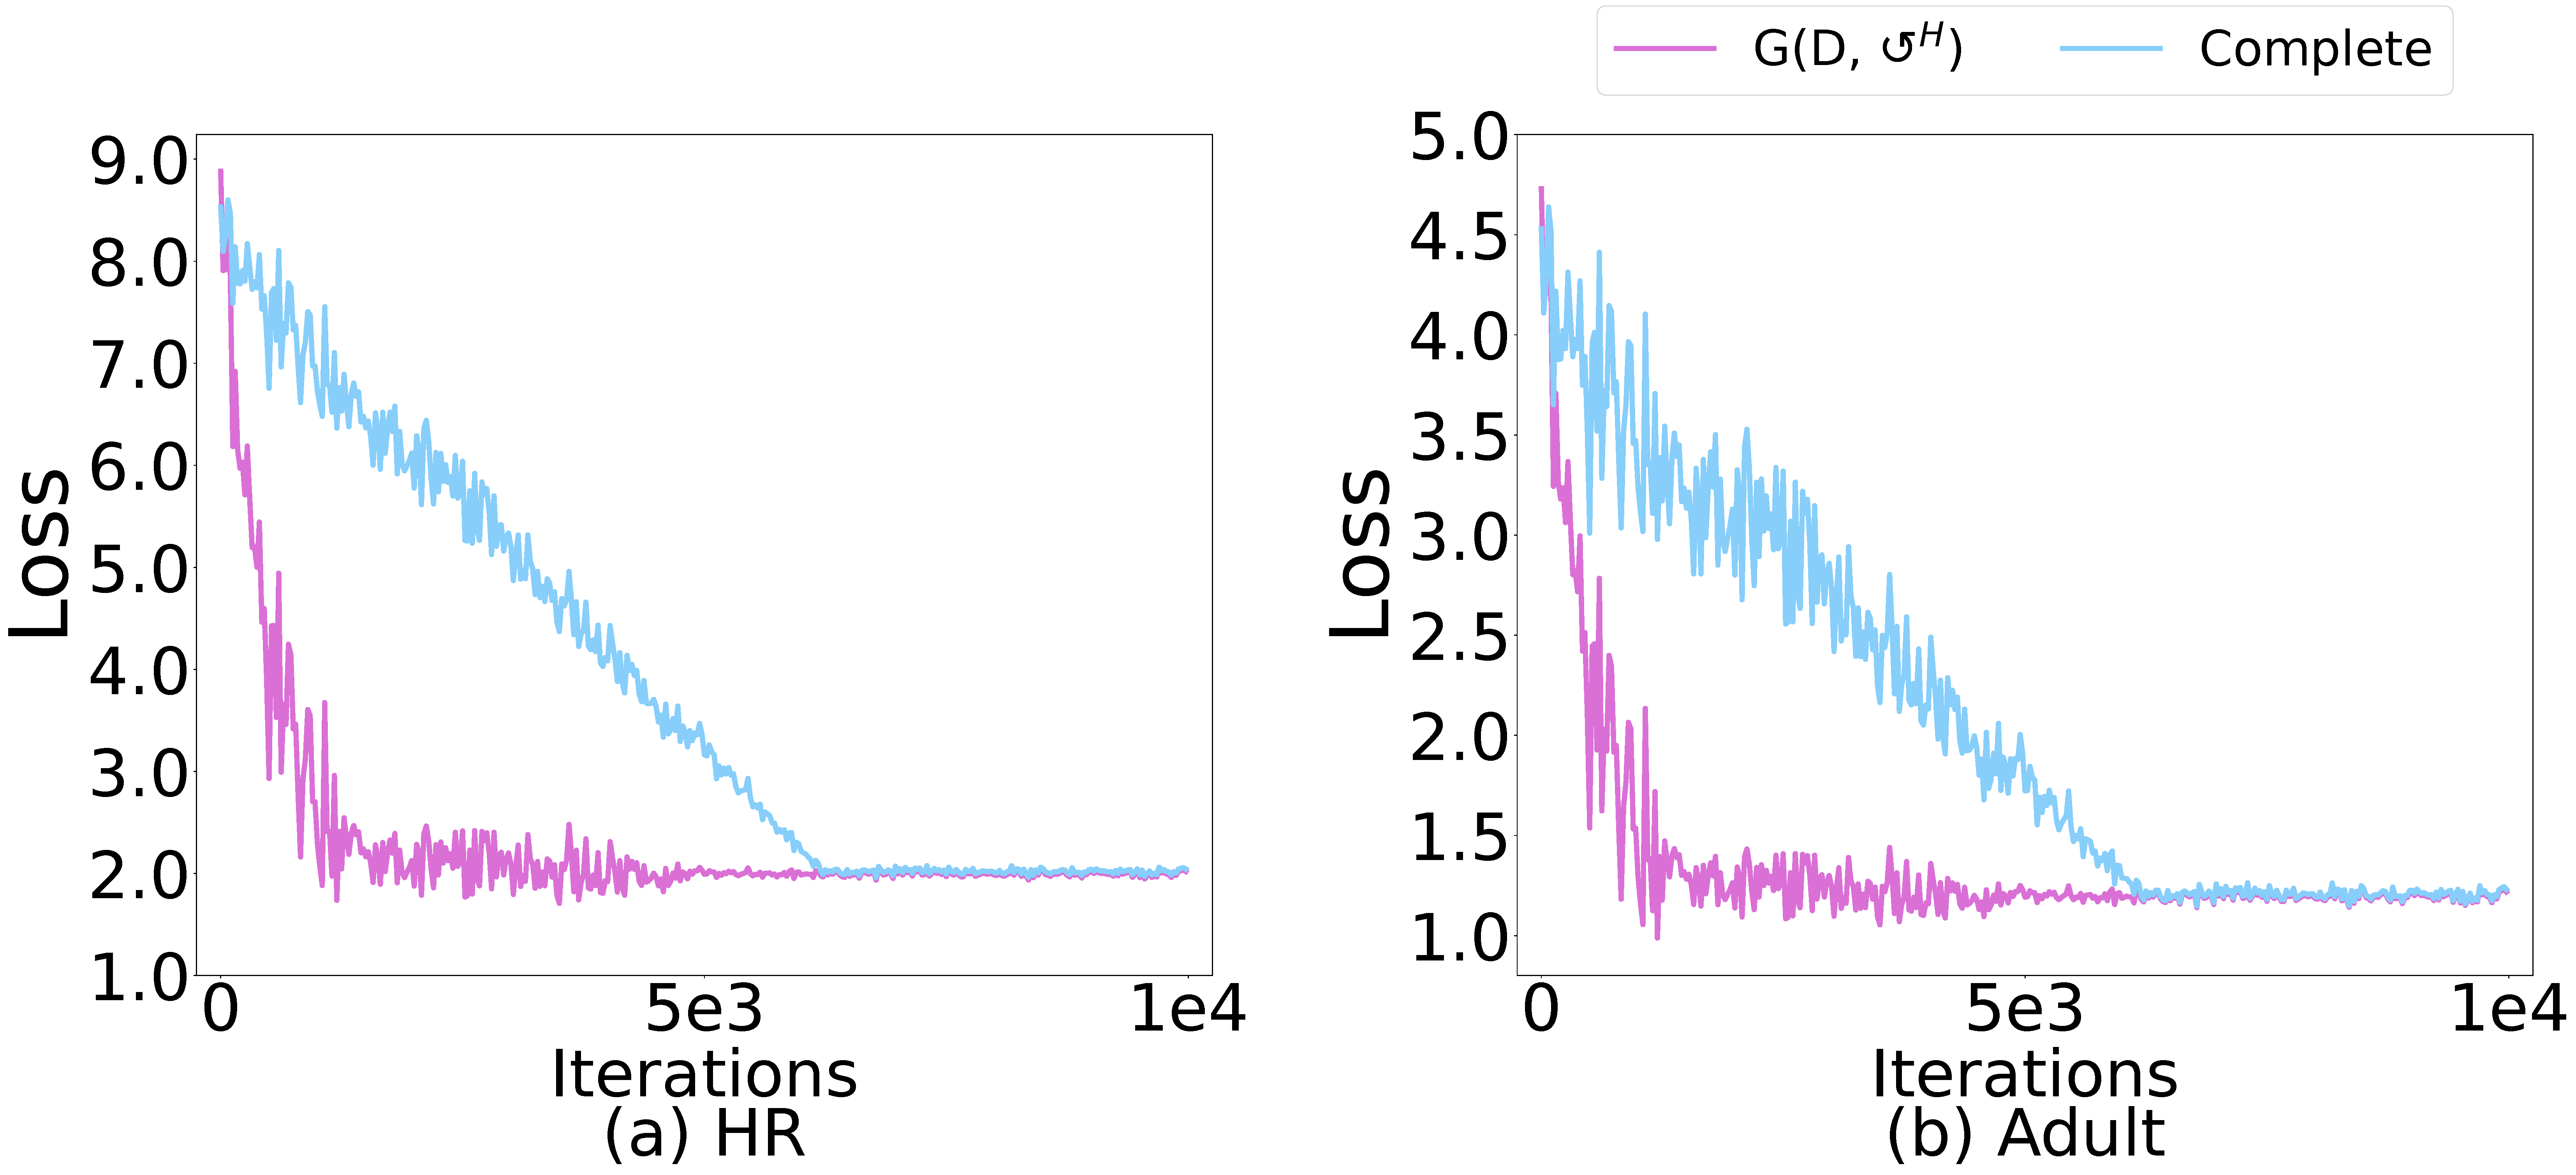
\includegraphics[width=\columnwidth]{figs/G}
	    \vspace{-1.5em}
		\caption{Loss of \ours.}
		\label{fig:real_loss_G}
	\end{minipage}
	\vspace*{-1em}   
\end{figure}

\begin{figure}[t]   
	\centering
	\begin{minipage}[t]{0.49\textwidth}
		\centering
		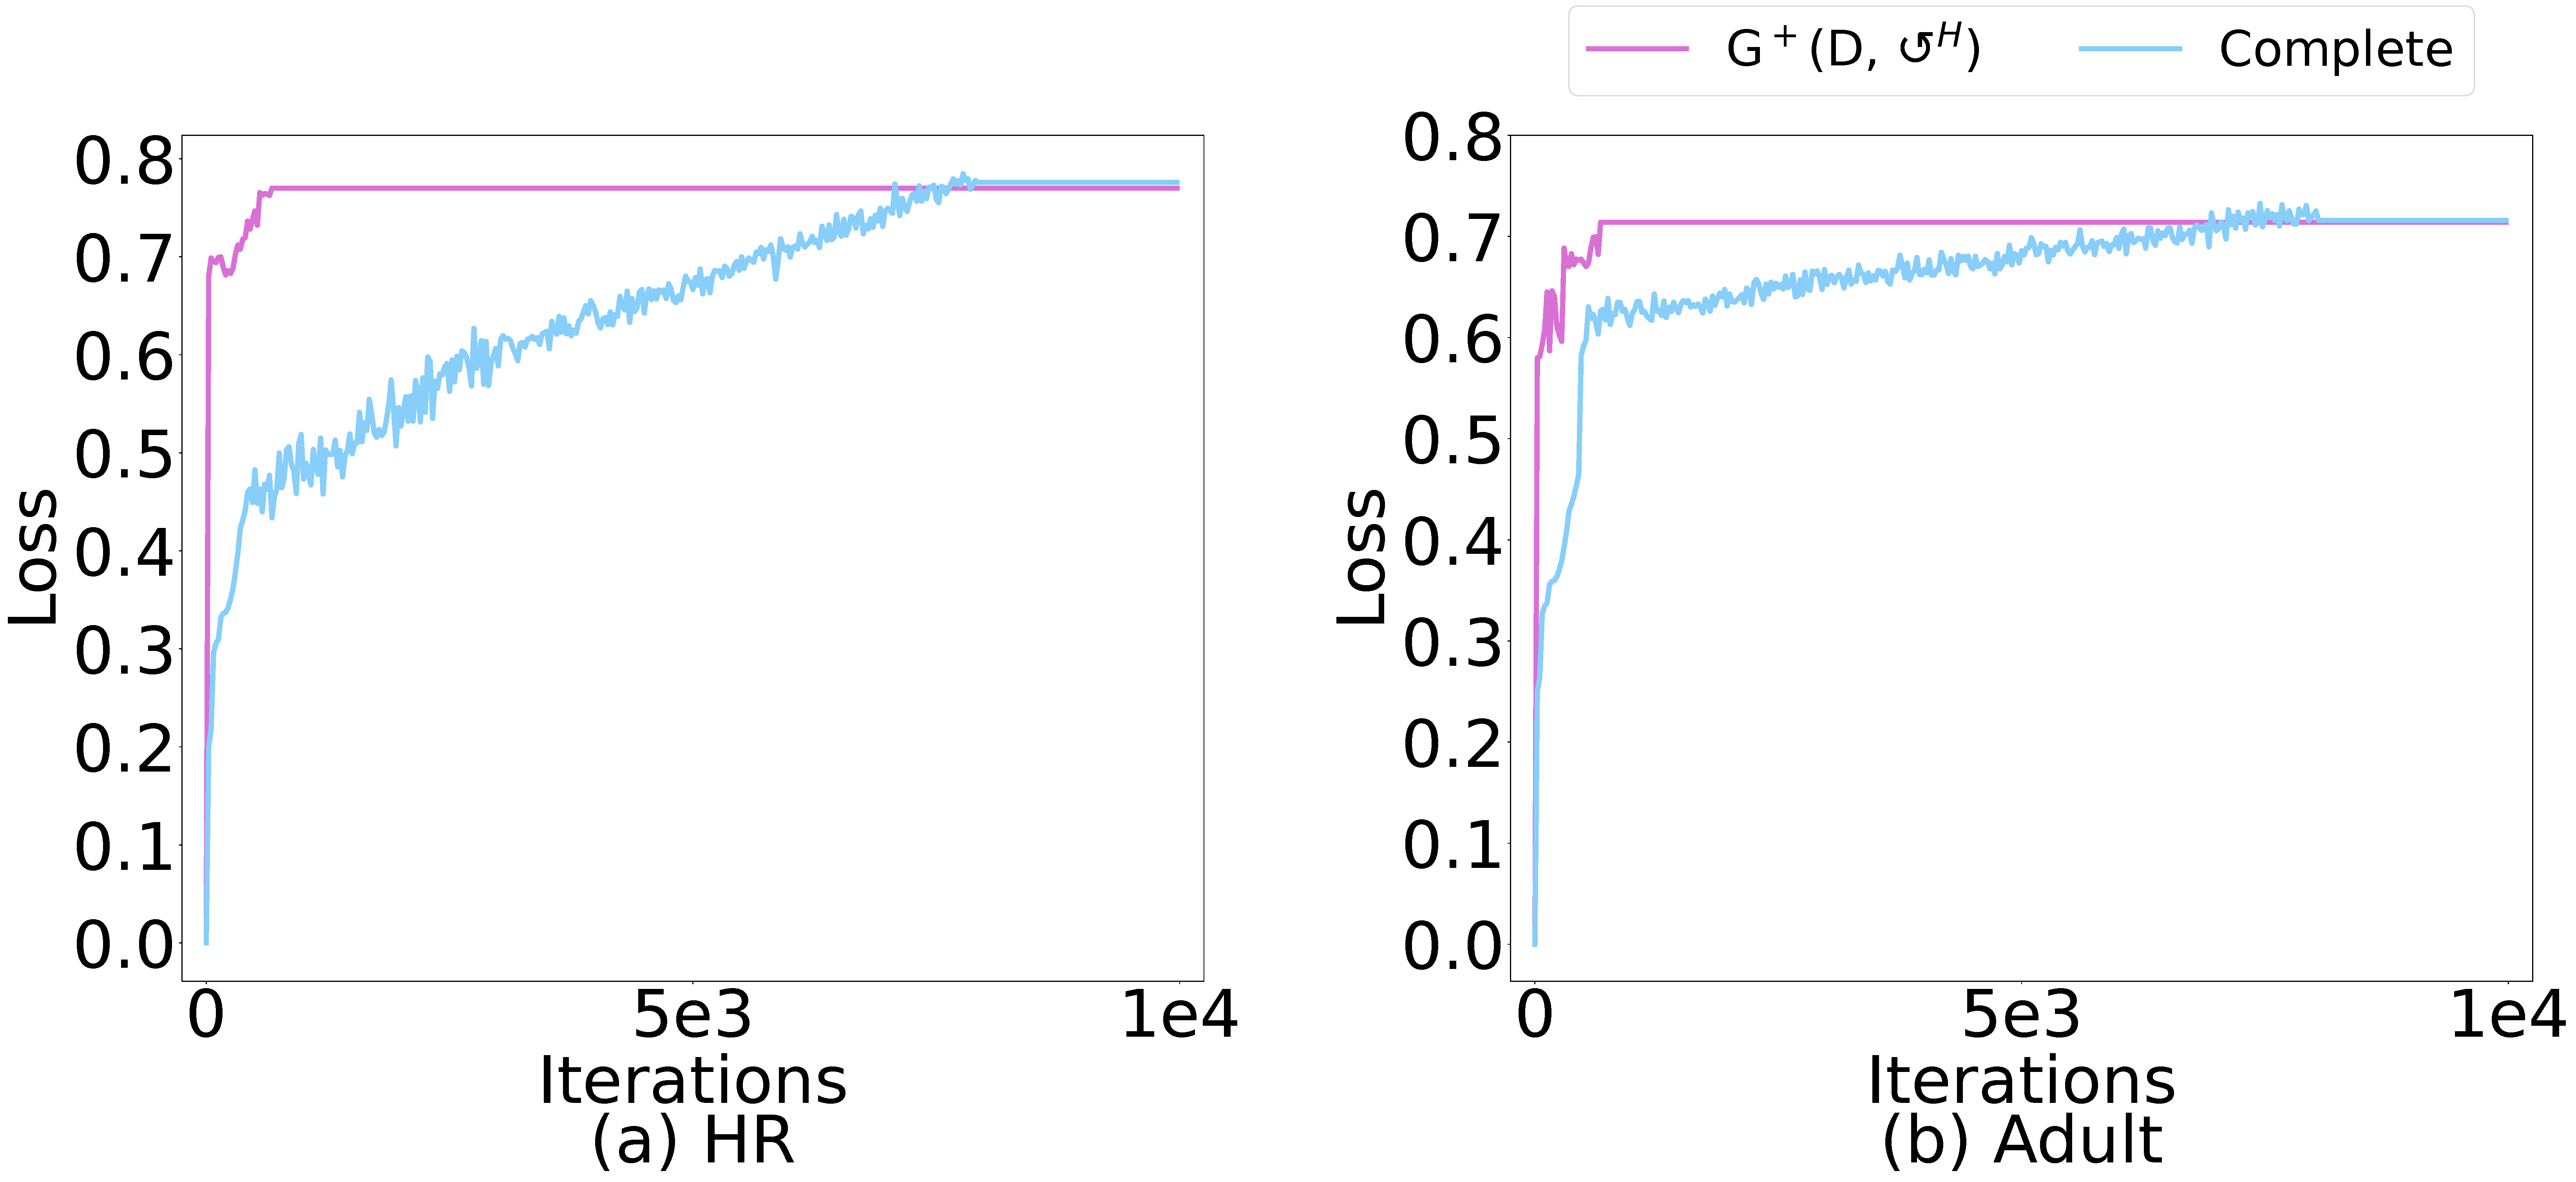
\includegraphics[width=\columnwidth]{figs/G+_a}
		\vspace{-1.5em}
		\caption{Convergence of \texttt{GoodCore}$^+$.}
		\label{fig:converge_G+}
	\end{minipage}
	\begin{minipage}[t]{0.49\textwidth}
		\centering
		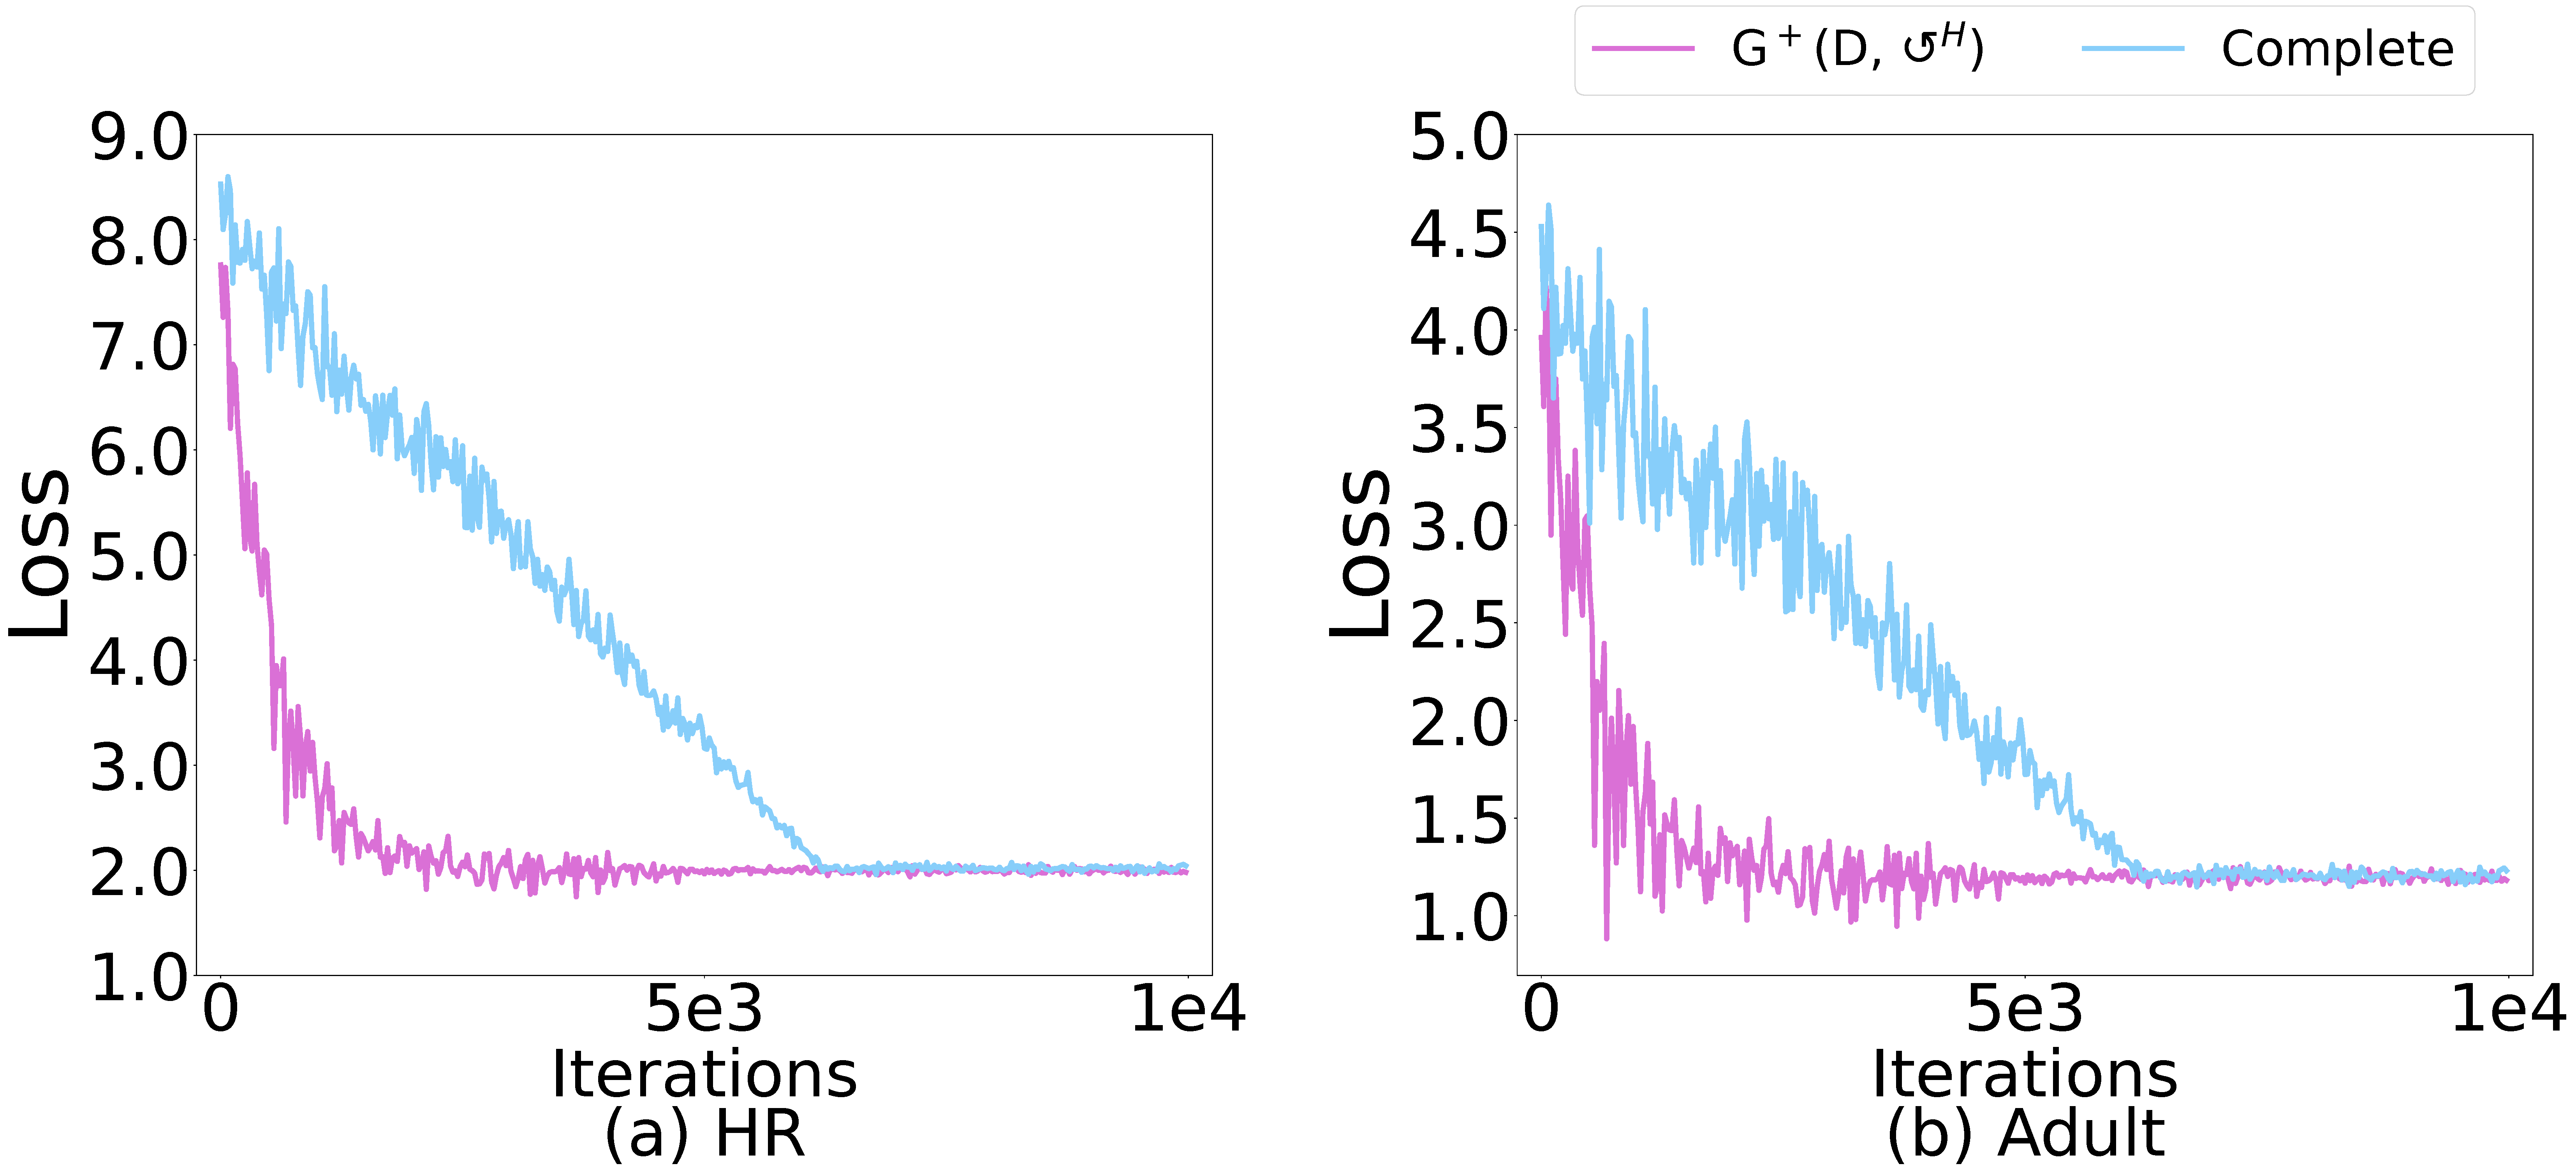
\includegraphics[width=\columnwidth]{figs/G+}
		\vspace{-1.5em}
		\caption{Loss of \texttt{GoodCore}$^+$.}
		\label{fig:real_loss_G+}
	\end{minipage}
	\vspace*{-1em}   
\end{figure}

In Section~\ref{sec:proof}, we have shown  the convergence rate of \ours theoretically. In this part, we test the convergence of training over the coreset ($\seven$) and entire data (\truth) empirically.  Figure~\ref{fig:converge_G} shows the test accuracy of two methods with the number of training iterations increasing. We can observe that on both datasets, training on the coreset converges much faster than training on the full data. 

For example, on dataset \adult, it takes $\sim$40 iterations for \ours to converge, which is  $180\times$ faster than {\truth}. This is because \ours has the same convergence rate with training over the entire dataset as discussed in the theoretical result of Section~\ref{sec:proof}, but the entire dataset (\eg  ~\adult) is $200\times$ (similar to $180\times$) larger than the coreset ($\rho=0.005$).
 That is, \ours converges with the same number of epochs  as training on the entire dataset. Since the size of coreset is much smaller, \ours is more efficient. Also, we can achieve competitive accuracy as training on full data by approximating the full gradient with a theoretical bound. 

Furthermore, we report the loss change to reflect the relation between  actual convergence rate and theoretical results. In Figure~\ref{fig:real_loss_G}, on dataset \hr, the initial loss is 8.4. According to the theoretical convergence rate $O(\frac{1}{\sqrt{k}})$ (this $k$ denotes the $k$-th epoch),  the loss should decrease to around 3.8 at the end of 5-th epoch ($\approx$ 3200-th iteration). Actually,  the  actual loss decreases to 3.25 at that time, which is close to the theoretical value.

We also test the convergence of \texttt{GoodCore}$^+$, as shown in Figure~\ref{fig:converge_G+} and 	\ref{fig:real_loss_G+}. The results  validate that the group-based method can also converge fast.

%\jks{We theoretically established the convergence rate of \ours$^+$. Then we empirically evaluate the convergence of training on the coreset ($\nine$) and the entire dataset (\truth) in Section~\ref{subsec:pq}. Figure~\ref{fig:converge_G+} depicts the test accuracy of both methods as the number of training iterations increases. It is evident that training on the coreset achieves faster convergence compared to training on the full dataset, observed across both datasets.
%For example, on dataset \adult, it takes $\sim$40 iterations for \ours$^+$ to converge, which is  $180\times$ faster than {\truth} and the same as $\seven$. This is because \ours$^+$ and \ours have the same convergence rate with training over the entire dataset, which are both $200\times$ (similar to $180\times$) smaller than the entire dataset. Consequently, \texttt{GoodCore}$^+$ converges within an equivalent number of epochs compared to training on the entire dataset. Given the substantially smaller size of the coreset, \ours$^+$ exhibits superior efficiency. Moreover, by approximating the full gradient using a theoretical bound, we can attain competitive accuracy akin to training on the complete dataset. }
 

%\jks{Alternatively, we also report the variations in loss to demonstrate the connection between the actual convergence speed and the theoretical results. As shown in Figure~\ref{fig:real_loss_G+}, on dataset \hr, the initial loss is 7.7. And the loss should decrease to around 3.5 at the end of 5-th epoch ($\approx$ 3200-th iteration) based on the theoretical convergence rate. Actually, the actual loss decreases to 3.04 at that time, which is close to the theoretical value.}